\documentclass[tikz, border=2pt]{standalone}
\usepackage{tikz,pgfplots}
\usepgfplotslibrary{colormaps}
\usepackage{tikz-3dplot}
\usepackage{amsmath,bm,array}
\usepackage{amsfonts,amsthm,titlesec}


\newcommand{\bbA}{\mathbb{A}}
\newcommand{\bbB}{\mathbb{B}}
\newcommand{\bbC}{\mathbb{C}}
\newcommand{\bbD}{\mathbb{D}}
\newcommand{\bbE}{\mathbb{E}}
\newcommand{\bbF}{\mathbbF}
\newcommand{\bbG}{\mathbb{G}}
\newcommand{\bbH}{\mathbb{H}}
\newcommand{\bbI}{\mathbb{I}}
\newcommand{\bbJ}{\mathbb{J}}
\newcommand{\bbK}{\mathbb{K}}
\newcommand{\bbL}{\mathbb{L}}
\newcommand{\bbM}{\mathbb{M}}
\newcommand{\bbN}{\mathbb{N}}
\newcommand{\bbO}{\mathbb{O}}
\newcommand{\bbP}{\mathbb{P}}
\newcommand{\bbQ}{\mathbb{Q}}
\newcommand{\bbR}{\mathbb{R}}
\newcommand{\bbS}{\mathbb{S}}
\newcommand{\bbT}{\mathbb{T}}
\newcommand{\bbU}{\mathbb{U}}
\newcommand{\bbV}{\mathbb{V}}
\newcommand{\bbW}{\mathbb{W}}
\newcommand{\bbX}{\mathbb{X}}
\newcommand{\bbY}{\mathbb{Y}}
\newcommand{\bbZ}{\mathbb{Z}}

\def\bfa{{\boldsymbol a}}
\def\bfb{{\boldsymbol b}}
\def\bfc{{\boldsymbol c}}
\def\bfd{{\boldsymbol d}}
\def\bfe{{\boldsymbol e}}
\def\bff{{\boldsymbol f}}
\def\bfg{{\boldsymbol g}}
\def\bfh{{\boldsymbol h}}
\def\bfi{{\boldsymbol i}}
\def\bfj{{\boldsymbol j}}
\def\bfk{{\boldsymbol k}}
\def\bfl{{\boldsymbol l}}
\def\bfm{{\boldsymbol m}}
\def\bfn{{\boldsymbol n}}
\def\bfo{{\boldsymbol o}}
\def\bfp{{\boldsymbol p}}
\def\bfq{{\boldsymbol q}}
\def\bfr{{\boldsymbol r}}
\def\bfs{{\boldsymbol s}}
\def\bft{{\boldsymbol t}}
\def\bfu{{\boldsymbol u}}
\def\bfv{{\boldsymbol v}}
\def\bfw{{\boldsymbol w}}
\def\bfx{{\boldsymbol x}}
\def\bfy{{\boldsymbol y}}
\def\bfz{{\boldsymbol z}}

\def\bfA{{\boldsymbol A}}
\def\bfB{{\boldsymbol B}}
\def\bfC{{\boldsymbol C}}
\def\bfD{{\boldsymbol D}}
\def\bfE{{\boldsymbol E}}
\def\bfF{{\boldsymbol F}}
\def\bfG{{\boldsymbol G}}
\def\bfH{{\boldsymbol H}}
\def\bfI{{\boldsymbol I}}
\def\bfJ{{\boldsymbol J}}
\def\bfK{{\boldsymbol K}}
\def\bfL{{\boldsymbol L}}
\def\bfM{{\boldsymbol M}}
\def\bfN{{\boldsymbol N}}
\def\bfO{{\boldsymbol O}}
\def\bfP{{\boldsymbol P}}
\def\bfQ{{\boldsymbol Q}}
\def\bfR{{\boldsymbol R}}
\def\bfS{{\boldsymbol S}}
\def\bfT{{\boldsymbol T}}
\def\bfU{{\boldsymbol U}}
\def\bfV{{\boldsymbol V}}
\def\bfW{{\boldsymbol W}}
\def\bfX{{\boldsymbol X}}
\def\bfY{{\boldsymbol Y}}
\def\bfZ{{\boldsymbol Z}}

\def\bf0{{\boldsymbol 0}}
\def\bfxi{{\boldsymbol \xi}}
\def\bfkappa{{\boldsymbol \kappa}}
\def\bfeps{{\boldsymbol \varepsilon}}
\def\bfeta{{\boldsymbol \eta}}
\def\bfphi{{\boldsymbol \varphi}}
\def\bfnu{{\boldsymbol \nu}}
\def\bfomega{{\boldsymbol \omega}}
\def\bfOmega{{\boldsymbol \Omega}}
\def\bfpsi{{\boldsymbol \psi}}
\def\bfchi{{\boldsymbol \chi}}
\def\bftau{{\boldsymbol \tau}}
\def\bfsigma{{\boldsymbol \sigma}}
\def\bfSigma{{\boldsymbol \Sigma}}

\def\Reyn{\mathrm{Re}}
\def\Bond{\mathrm{Bo}}
\def\Cap{\mathrm{Ca}}
\def\Sto{\mathrm{St}}


\begin{document}
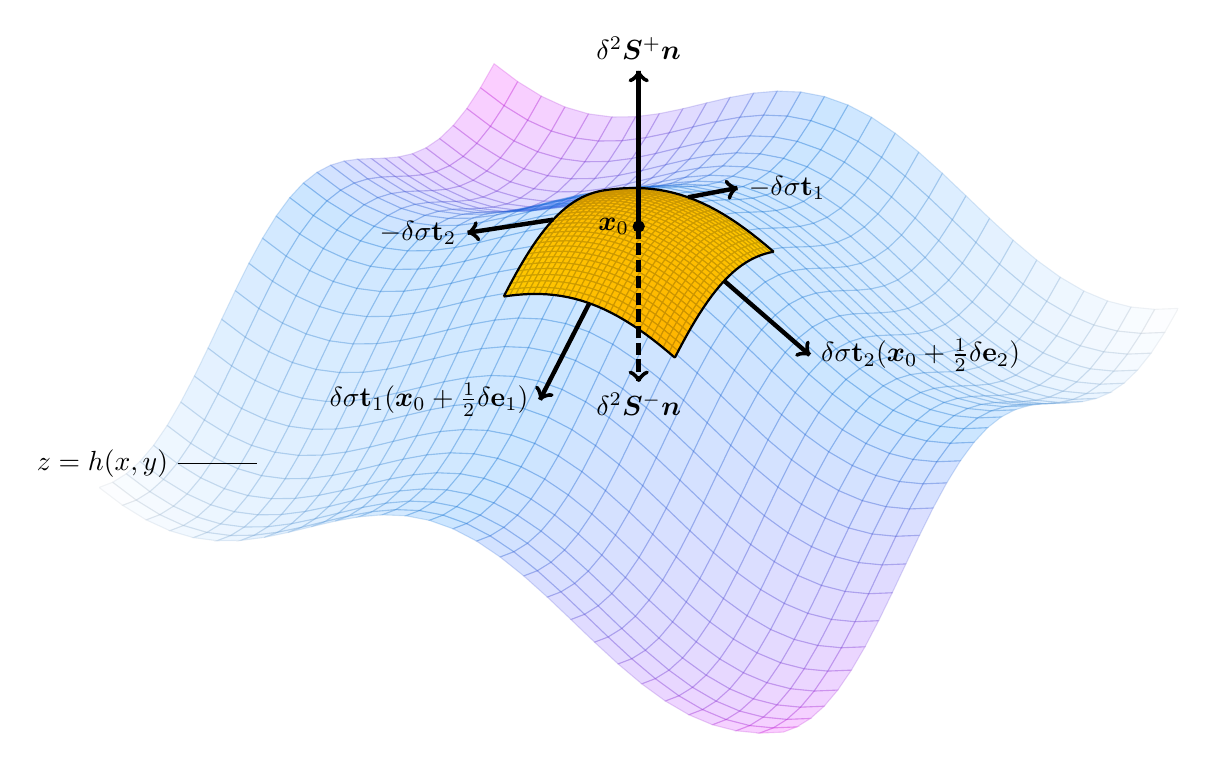
\begin{tikzpicture}
  \begin{axis}[
      hide axis,
      scale=2,
      view={120}{65},
      xmin=-4,xmax=4,
      ymin=-4,ymax=4,
      zmin=-2.2,zmax=2.2,
      trig format plots=rad,
      ]
      \addplot3 [ surf, colormap/cool, domain=-4:4, domain y=-4:4,
              samples=30, samples y=30,
              variable=\u, variable y=\v,
              point meta=u*v,opacity=0.2]
            ( {u}, {v}, {cos(u) + cos(v)} );

  % Plot surface
  \addplot3 [ surf, domain=-1:1, domain y=-1:1,
              samples=30, samples y=30,
              variable=\u, variable y=\v,
              point meta=u*v]
            ( {u}, {v}, {cos(u) + cos(v)} );
  
  % Plot section of surface
  \addplot3[black, thick, variable=\t, domain=-1:1, samples y=1] ( 1, {t}, {cos(1) + cos(t)});
  \addplot3[black, thick, variable=\t, domain=-1:1, samples y=1] ( -1, {t}, {cos(1) + cos(t)});
  \addplot3[black, thick, variable=\t, domain=-1:1, samples y=1] ( {t}, 1, {cos(1) + cos(t)});
  \addplot3[black, thick, variable=\t, domain=-1:1, samples y=1] ( {t}, -1, {cos(1) + cos(t)});

  \draw[fill=black] (axis cs:0,0,2) circle[radius=2pt] node[left] {$\bfx_0$};
  
  % Plot normal stresses
  \addplot3[->, ultra thick, black, variable=\t,domain=0:1,samples=2] (0,0,{2+3*t}) node[above] {$\delta^2\bfS^+\bfn$};
  \addplot3[->, ultra thick, black, dashed, dash pattern=on 2pt off 4pt, variable=\t,domain=0:1,samples=2] (0,0,{2-3*t}) node[below] {$\delta^2\bfS^-\bfn$};

  % Plot surface tension forces
  \addplot3[->, ultra thick, black, variable=\t,domain=0:1,samples=10] (1+t,0,{cos(1)+1-t*sin(1)}) node[left] {$\delta\sigma\mathbf{t}_1(\bfx_0+\tfrac12\delta \mathbf{e}_1)$};
  \addplot3[->, ultra thick, black, variable=\t,domain=0:1,samples=10] (-1-t,0,{cos(1)+1-t*sin(1)}) node[right] {$-\delta \sigma\mathbf{t}_1$};
  \addplot3[->, ultra thick, black, variable=\t,domain=0:1,samples=10] (0,1+t,{cos(1)+1-t*sin(1)}) node[right] {$\delta \sigma \mathbf{t}_2(\bfx_0+\tfrac12\delta \mathbf{e}_2)$};
  \addplot3[->, ultra thick, black, variable=\t,domain=0:1,samples=10] (0,-1-t,{cos(1)+1-t*sin(1)}) node[left] {$-\delta\sigma\mathbf{t}_2$};
  \end{axis}

  \draw[thin, black] (1,4)  node[left] {$z=h(x,y)$} -- (2,4);
\end{tikzpicture}

\end{document}